\section{Introduction}

This \cgal\ component implements methods to analyze and process unorganized 3D point sets. The input is an unorganized 3D point set, possibly with attributes such as unoriented or oriented normals. This point set can be analyzed to measure certain geometric properties such as average spacing between the points and their $K$ nearest neighbors. We can furthermore process the point set with functions devoted to the simplification, outlier removal, smoothing, normal estimation and normal orientation. 


The processing of point sets is often needed by applications dealing with measurement data, such as surface reconstruction from laser scanned data (see Figure \ref{Point_set_processing_3-fig-introduction}).

% TOFIX: left and right with same viewpoint.

% Insert image introduction.jpg/eps
\begin{center}
    \label{Point_set_processing_3-fig-introduction}
    % Image
    \begin{ccTexOnly}
        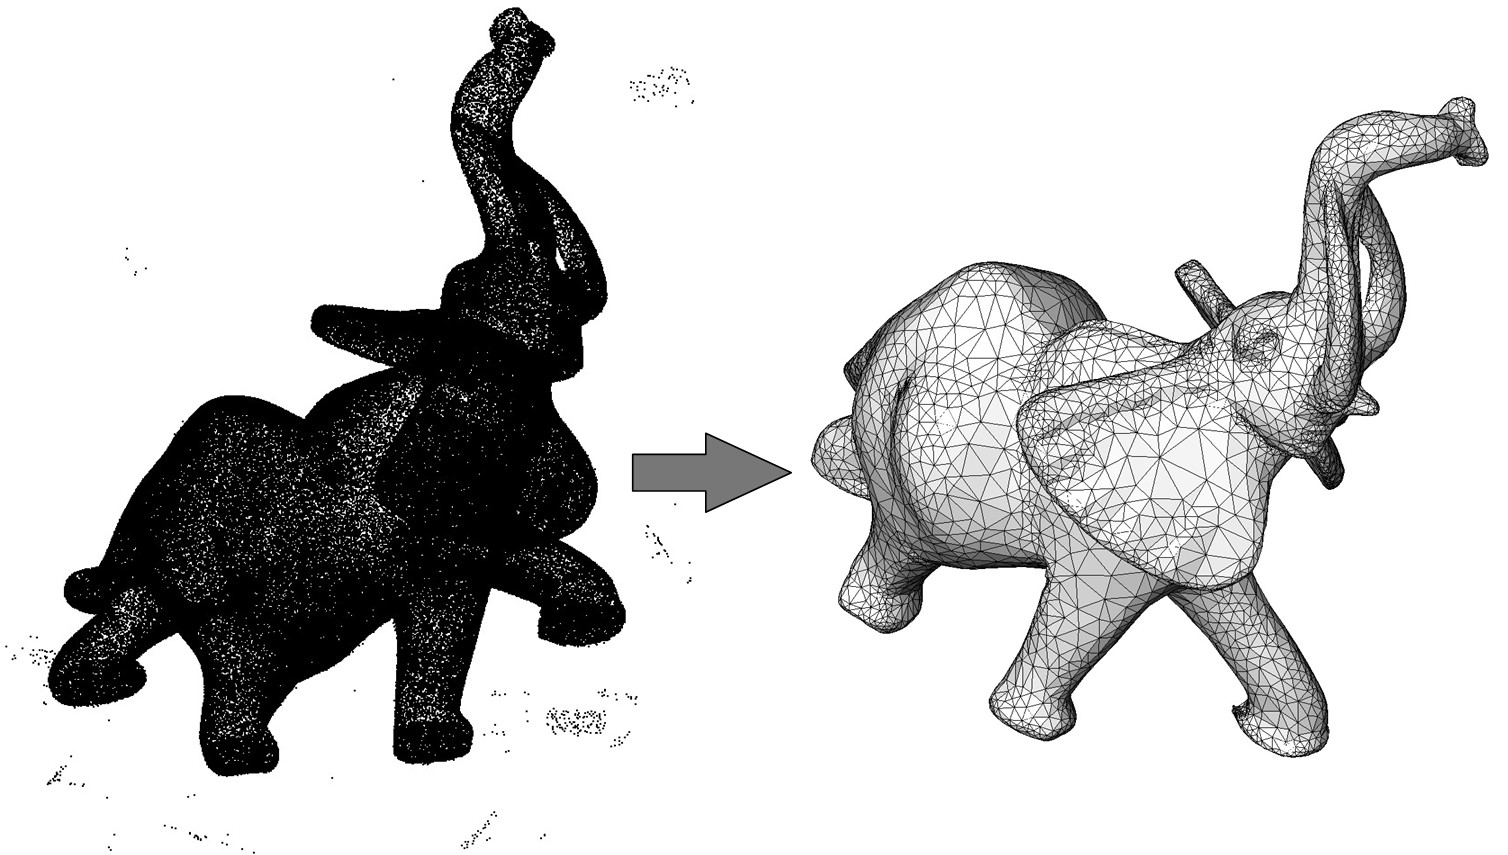
\includegraphics[width=1.0\textwidth]{Point_set_processing_3/introduction} % omit .eps suffix
    \end{ccTexOnly}
    \begin{ccHtmlOnly}
        <img width="90%" border=0 src="./introduction.jpg"><P>
    \end{ccHtmlOnly}
    % Title
    \begin{figure}[h]
        \caption{Point set processing.
                 Left: 275K points sampled on an elephant with
                 a Minolta laser scanner.
                 Right: point set after clean-up and
                 simplification to 17K points.}
    \end{figure}
\end{center}

In the context of surface reconstruction we can replace the elements of this component along the common surface reconstruction pipeline which involves the following steps: 1) Scanning and scan alignment to produce a set of points or points with normals (alignment is not yet covered in \cgal); 2) Outlier removal; 3) Simplification to reduce the number of input points; 4) Smoothing to reduce noise in the input data; 5) Normal estimation and orientation when the normals are not already provided by the acquisition device; and 6) Surface reconstruction. Chapter \ccc{Surface_reconstruction_points_3} \ref{chap:surface_reconstruction_points_3} deals with surface reconstruction from point sets with normal attributes.

Figure \ref{Point_set_processing_3-fig-pipeline} illustrates this pipeline.

% Insert image pipeline.jpg/eps
\begin{center}
    \label{Point_set_processing_3-fig-pipeline}
    % Image
    \begin{ccTexOnly}
        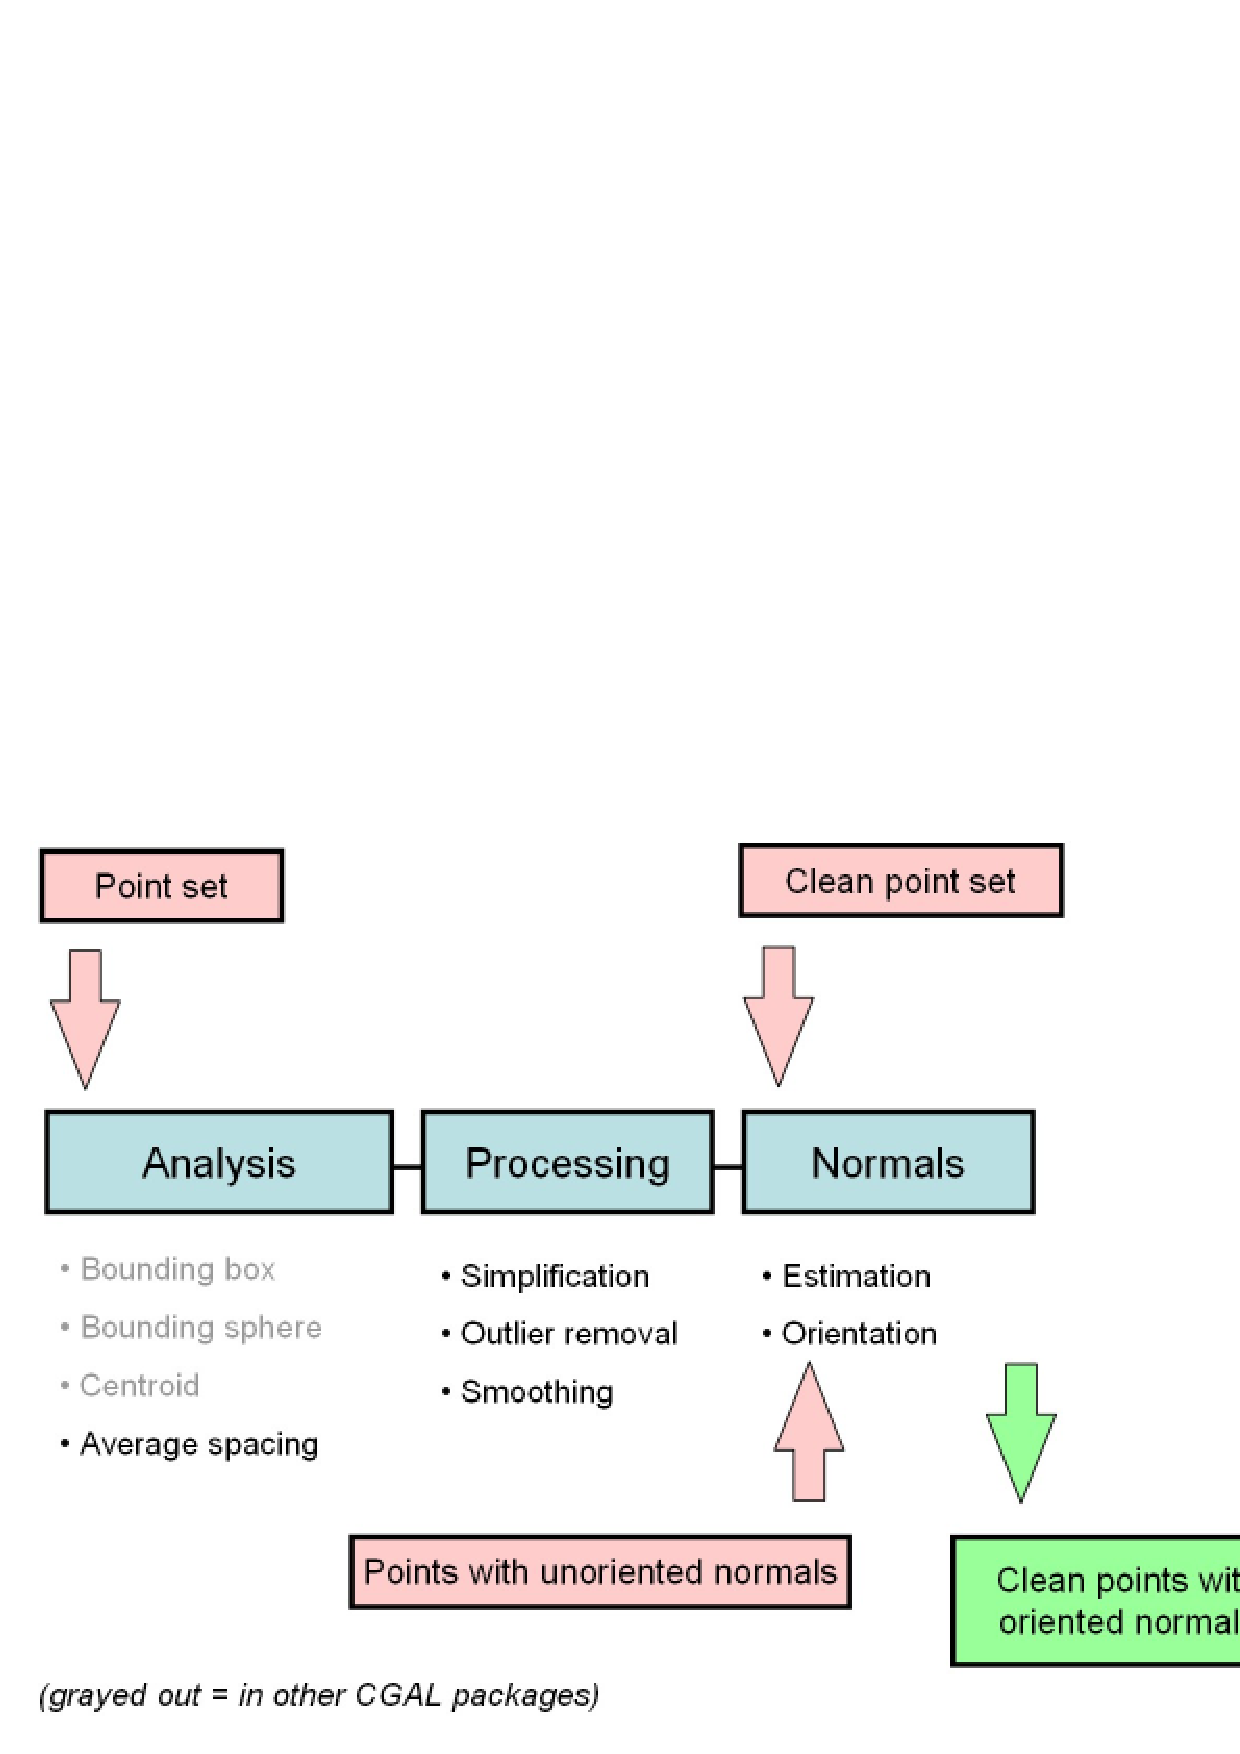
\includegraphics[width=0.8\textwidth]{Point_set_processing_3/pipeline} % omit .eps suffix
    \end{ccTexOnly}
    \begin{ccHtmlOnly}
        <img width="65%" border=0 src="./pipeline.jpg"><P>
    \end{ccHtmlOnly}
    % Title
    \begin{figure}[h]
        \caption{Point set processing pipeline for surface reconstruction.}
    \end{figure}
\end{center}


